\documentclass[a4paper, 12pt]{article}%тип документа

%%%Библиотеки
	%\usepackage[warn]{mathtext}	
	\usepackage[T2A]{fontenc} % кодировка
	\usepackage[utf8]{inputenc} % кодировка исходного текста
	\usepackage[english,russian]{babel} % локализация и переносы
	\usepackage{caption}
	\usepackage{listings}
	\usepackage{amsmath,amsfonts,amssymb,amsthm,mathtools}
	\usepackage{wasysym}
	\usepackage{graphicx}%Вставка картинок правильная
	\usepackage{float}%"Плавающие" картинки
	\usepackage{wrapfig}%Обтекание фигур (таблиц, картинок и прочего)
	\usepackage{fancyhdr} %загрузим пакет
	\usepackage{lscape}
	\usepackage{xcolor}
	\usepackage[normalem]{ulem}
	\usepackage{hyperref}

%%%Конец библиотек




%%%Настройка ссылок
	\hypersetup
	{
		colorlinks=true,
		linkcolor=blue,
		filecolor=magenta,
		urlcolor=blue
	}
%%%Конец настройки ссылок


%%%Настройка колонтитулы
	\pagestyle{fancy}
	\fancyhead{}
	\fancyhead[L]{Лабораторная работа}
	\fancyhead[R]{Талашкевич Даниил, группа Б01-009}
	\fancyfoot[C]{\thepage}
%%%конец настройки колонтитулы



							\begin{document}
						%%%%Начало документа%%%%


%%%Начало титульника
\begin{titlepage}

	\newpage
	\begin{center}
		\normalsize Московский физико-технический институт \\(госудраственный 			университет)
	\end{center}

	\vspace{6em}

	\begin{center}
		\Large Лабораторная работа по электричеству\\
	\end{center}

	\vspace{1em}

	\begin{center}
		\large \textbf{Петля гистерезиса (динамический метод) [3.4.5]}
	\end{center}

	\vspace{2em}

	\begin{center}
		\large Талашкевич Даниил Александрович\\
		Группа Б01-009
	\end{center}

	\vspace{\fill}

	\begin{center}
	Долгопрудный \\2021
	\end{center}
	
\end{titlepage}
%%%Конец Титульника



%%%Настройка оглавления и нумерации страниц
	\thispagestyle{empty}
	\newpage
	\tableofcontents
	\newpage
	\setcounter{page}{1}
%%%Настройка оглавления и нумерации страниц


					%%%%%%Начало работы с текстом%%%%%%
					
\textbf{Цель работы:} исследование предельных петель гистерезиса и начальных кривых намагничивания для нескольких ферромагнитных образцов; определение магнитных характеристик материалов, чувствительность каналов $X$ и $Y$ осциллографа и постоянную времени $\tau$ интегрирующей цепочки.\\

\textbf{Используемое оборудование:} автотрансформатор, понижающий трансформатор, амперметр и вольтметр, резистор, делитель напряжения, интегрирующая цепочка, электронный осциллограф, тороидальные образцы с двумя обмотками.
                    
\section{Теоретическое введение}

Исследуемый сигнал подается на вход $X$; длина $2x$ горизонтальной черты, наблюдаемой на экране, характеризует удвоенную амплитуду сигнала. 

Если известна чувствительность усилителя $K_x$ в вольтах на деление шкалы экрана, то удвоенная амплитуда напряжения определяется произведением
\[2U_{X, 0} = 2x \cdot K_x\]
Напряжение, подаваемое на вход $Y$ определяется аналогично. 

Калибровку осей осциллографа можно использовать для построения кривой гистерезиса в координатах $B$ и $H$:

Зная величину сопротивления $R_0$, с которого снимается сигнал, можно определить чувствительность канала по току $K_{XI} = \dfrac{K_x}{R_0}$ [A/дел]; затем, используя формулу 
\begin{equation}
H = \dfrac{IN_0}{2\pi R}
\end{equation}
определить цену деления шкалы в A/м.

Используя формулу 
\begin{equation}
B = \dfrac{R_{\text{и}}C_{\text{и}}U_{\text{вых}}}{SN_{\text{и}}}
\end{equation}
можно рассчитать цену деления вертикальной шкалы в теслах.

\section{Экспериментальная установка}

Действующее значение переменного тока в обмотке $N_0$ измеряется амперметром $A$. Последовательно с амперметром включено сопротивление $R_0$, напряжение с которого подается на вход $X$ электронного осциллографа. Это напряжение пропорционально току в обмотке $N_0$, а следовательно и напряженности $H$ магнитного поля в образце.

Для измерения магнитной индукции $B$ с измерительной обмотки $N_{\text{и}}$ на вход интегрирующей $RC$-цепочки подается напряжение $U_{\text{и}}(U_{\text{вх}})$, пропорциональное $\dot{B}$, а, с выхода снимается напряжение $U_{\text{с}}(U_{\text{вых}})$, пропорциональное величине $B$, а подается на вход $Y$.


\begin{figure}[h!]
    \centering
	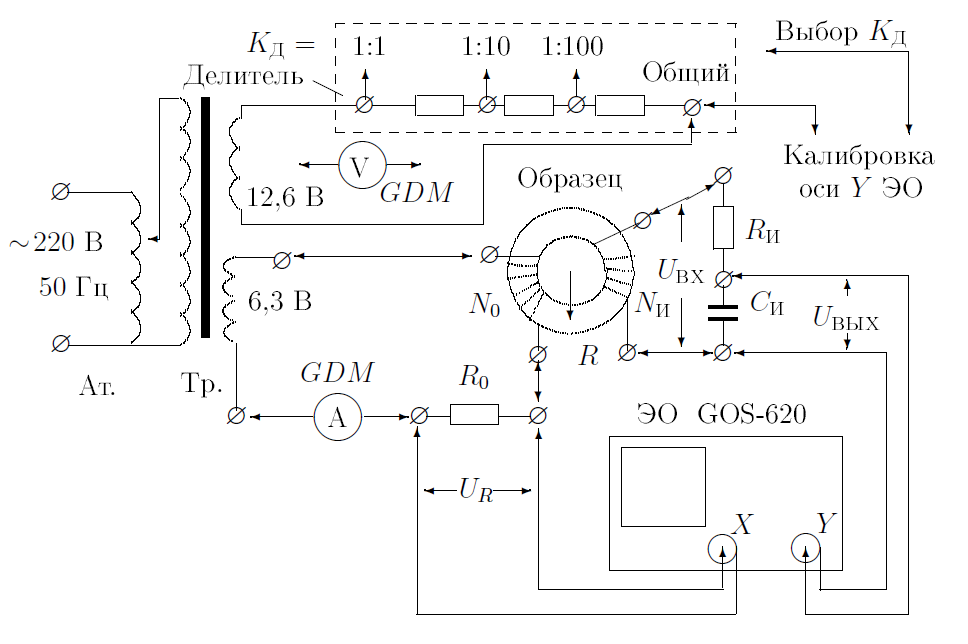
\includegraphics[width = \textwidth]{1.png}
    \caption{Схемы экспериментальных установок}
    \label{scheme}
\end{figure}


\section{Ход работы}


\section{Обработка результатов}


\section{Вывод}
 
\section{Литература}

\begin{enumerate}

\item \textbf{Лабораторный практикум по общей физике:} Учебное пособие. В трех томах. Т. 2. Электричество и магнетизм /Гладун А.Д., Александров Д.А., Берулёва Н.С. и др.; Под ред. А.Д. Гладуна - М.: МФТИ, 2007. - 280 с.

\end{enumerate}		
		


\end{document}